\subsection{Real-world data for simulation}

To do our numerical simulations, we will first consider the thermal conducitivty, density and heat capacity to be constants, we divide by $\rho c_p$ in \eqref{eq:heat} to get 
\begin{equation*}
    \theta_t - \alpha \nabla \cdot (\nabla \theta) = 0 \quad \text{in $\Omega \times (0,T)$ }
\end{equation*}
Here $\alpha = \frac{k}{\rho c_p}$ is the Thermal diffusivity. To do a simulation we can set $\alpha = 3.352 mm^2/s$ to represents stainless steel, one could also simulate other materials by choosing other values of $\alpha$. To represent iron one set $\alpha_{iron} = 23 mm^2/s$. Furthermore we need the thermal conducitivity as it appears in the boundary conditions. Our choice of parameters is shown in Table \ref{tab:chosenParam}.
\begin{table}[h]
    \centering
    \caption{Parameters used for numerical simulation of the rolling of steel process.}
    \begin{tabular}{c|c}
    $\text{Parameter}$ & $\text{SI-unit}$ \\
    \hline
       $k$& $\SI{50.2}{\joule\per\metre\per\second\per\kelvin}$ \\
        $c_p$ & $\SI{460.5}{\joule\per\kilogram\per\kelvin}$ \\
        $\rho$ & $\SI{8500}{\kilogram\per\metre\cubed}$ \\
        $\theta_w$ & $\SI{20}{\celsius}$ \\
        $\theta_d$ & $\SI{700}{\celsius}$ \\
    \end{tabular}
    \label{tab:chosenParam}
\end{table}

Simulations using the parameters of Table \ref{tab:chosenParam} are shown in Figure \ref{fig:state_simulations}. These simulations were produced using a finite element method (FEM) as implemented in the Python package \verb|FEniCS| \cite{fenics}. We observe that in Figure \ref{fig:state_simulations_a} the temperature is steadily decreasing, as one would expect when continously applying a coolant to the steel. In Figure \ref{fig:state_simulations_b}, however, all of the cooling seems to happen somewhere between $t=\SI{2}{\second}$ and $t=\SI{4}{\second}$. Again, this agrees with the intuition of applying almost no coolant at the beginning or end of the cooling cycle, and maximum coolant (i.e. $u=1$) at $t=\SI{3}{\second}$. The temperatures achieved also seem to agree with values found in the literature. Thus, we conclude that the parameters we have chosen are reasonable, and that the model and the simulation of the model both perform well.
\begin{figure}
    \makebox[\linewidth]{
        \centering
    \begin{subfigure}[t]{3in}
        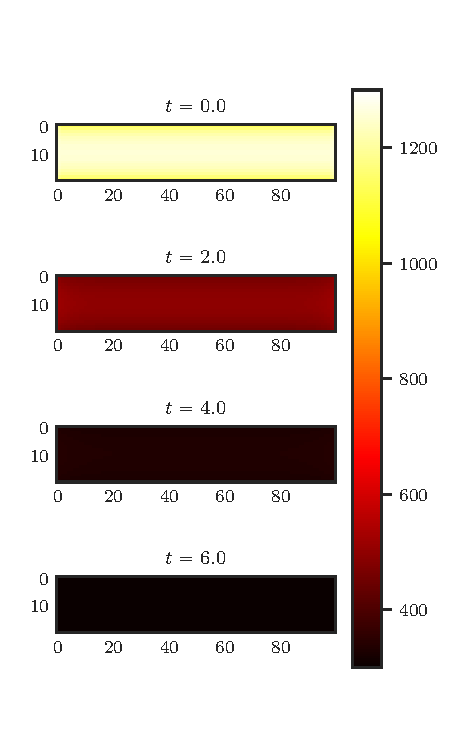
\includegraphics{figures/constant_u_state.pdf}
        \caption{Using the control $u(t)=1$.}
        \label{fig:state_simulations_a}
    \end{subfigure}
    ~
    \begin{subfigure}[t]{3in}
        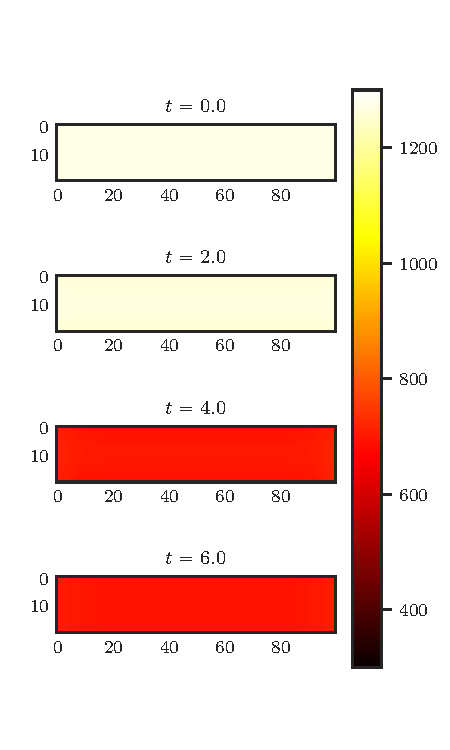
\includegraphics{figures/gaussian_u_state.pdf}
        \caption{Here, the control is $u(t) = \exp{\left(-\left(6(t-3)/10\right)^2\right)}$; a Gaussian centered around $t=3$.}
        \label{fig:state_simulations_b}
    \end{subfigure}
    }
    \caption{Simulations using the parameters given in Table \ref{tab:chosenParam}. In addition, the initial temperature of the steel was set to \SI{1300}{\celsius}. The control $u$ used is indicated in each figure caption.}
    \label{fig:state_simulations}
\end{figure}

\subsection{Improvements on the model}

A real-world simulation for the optimal cooling process of dual phase steels (DP steels) and in particular of the type Molydbenum-Magnesium in a rolling steel process can be modelled by choosing parameter with the value 
\begin{align*}
    \theta_d = \SI{680}{\celsius} \\
\end{align*}

One can furthermore make the model more realistic by as in \cite{DPSteelOverview} by coupling the semilinear heat equation with an ordinary differential equation that describe the evolution of steel microstructure during the cooling process. Then one consider the optimal control problem for the controlled cooling of steel profiles in order to obtain a desired temperature and a phase distribution in the steel. Such a phase transformation can in general be described by an initial value problem of the form 
\begin{align*}
    \frac{\partial f}{\partial t} = G(f,\theta ) \\
    f_{t=0} = 0
\end{align*}
Here f is a volume fraction of the new phase, G is typically a nonlinear function of its arguments. Then one can modify the heat equation to include a right-hand side term $\rho L \frac{\partial f}{\partial t}$, where $L$ is latent heat, hence the term describes realese of heat due to the phase transformation. Furthermore one have a desired phase distribution one want to obtain, denoted $f_d(x)$ one then modify the cost functional as well to obtain an approximation to the desired phase distribution. 